\chapter{Evaluation \& Testing}\label{ch:Evaluation}

\section{Exploratory Data Analysis}
\subsection{Data Overview}
Description of each dataset (refer to graphs as appendices)- Replacement of n/a value to mean values

\subsection{Class distribution}


\begin{table}[ht]
\centering
\begin{tabular}{lrl}
  \hline
Dataset & Percentage & Category \\ 
  \hline
Cervical\_Cancer & 95.45 & Majority Class \\ 
  Cervical\_Cancer & 4.55 & Minority Class \\ 
  Breast\_Cancer & 62.74 & Majority Class \\ 
  Breast\_Cancer & 37.26 & Minority Class \\ 
  Liver\_Disease & 71.36 & Majority Class \\ 
  Liver\_Disease & 28.64 & Minority Class \\ 
  Diabetes & 65.10 & Majority Class \\ 
  Diabetes & 34.90 & Minority Class \\ 
  Lower\_Back\_Pain & 32.26 & Majority Class \\ 
  Lower\_Back\_Pain & 67.74 & Minority Class \\ 
  Lower\_Back\_Pain(modified) & 87.72 & Majority Class \\ 
  Lower\_Back\_Pain(modified) & 12.28 & Minority Class \\ 
  Heart\_Attack & 63.95 & Majority Class \\ 
  Heart\_Attack & 36.05 & Minority Class \\ 
  Heart\_Attack(modified) & 94.95 & Majority Class \\ 
  Heart\_Attack(modified) & 5.05 & Minority Class \\ 
  Autism & 73.15 & Majority Class \\ 
  Autism & 26.85 & Minority Class \\ 
  Fertility & 88.00 & Majority Class \\ 
  Fertility & 12.00 & Minority Class \\ 
   \hline
\end{tabular}
\end{table}

\begin{figure}[H]
    \centering
    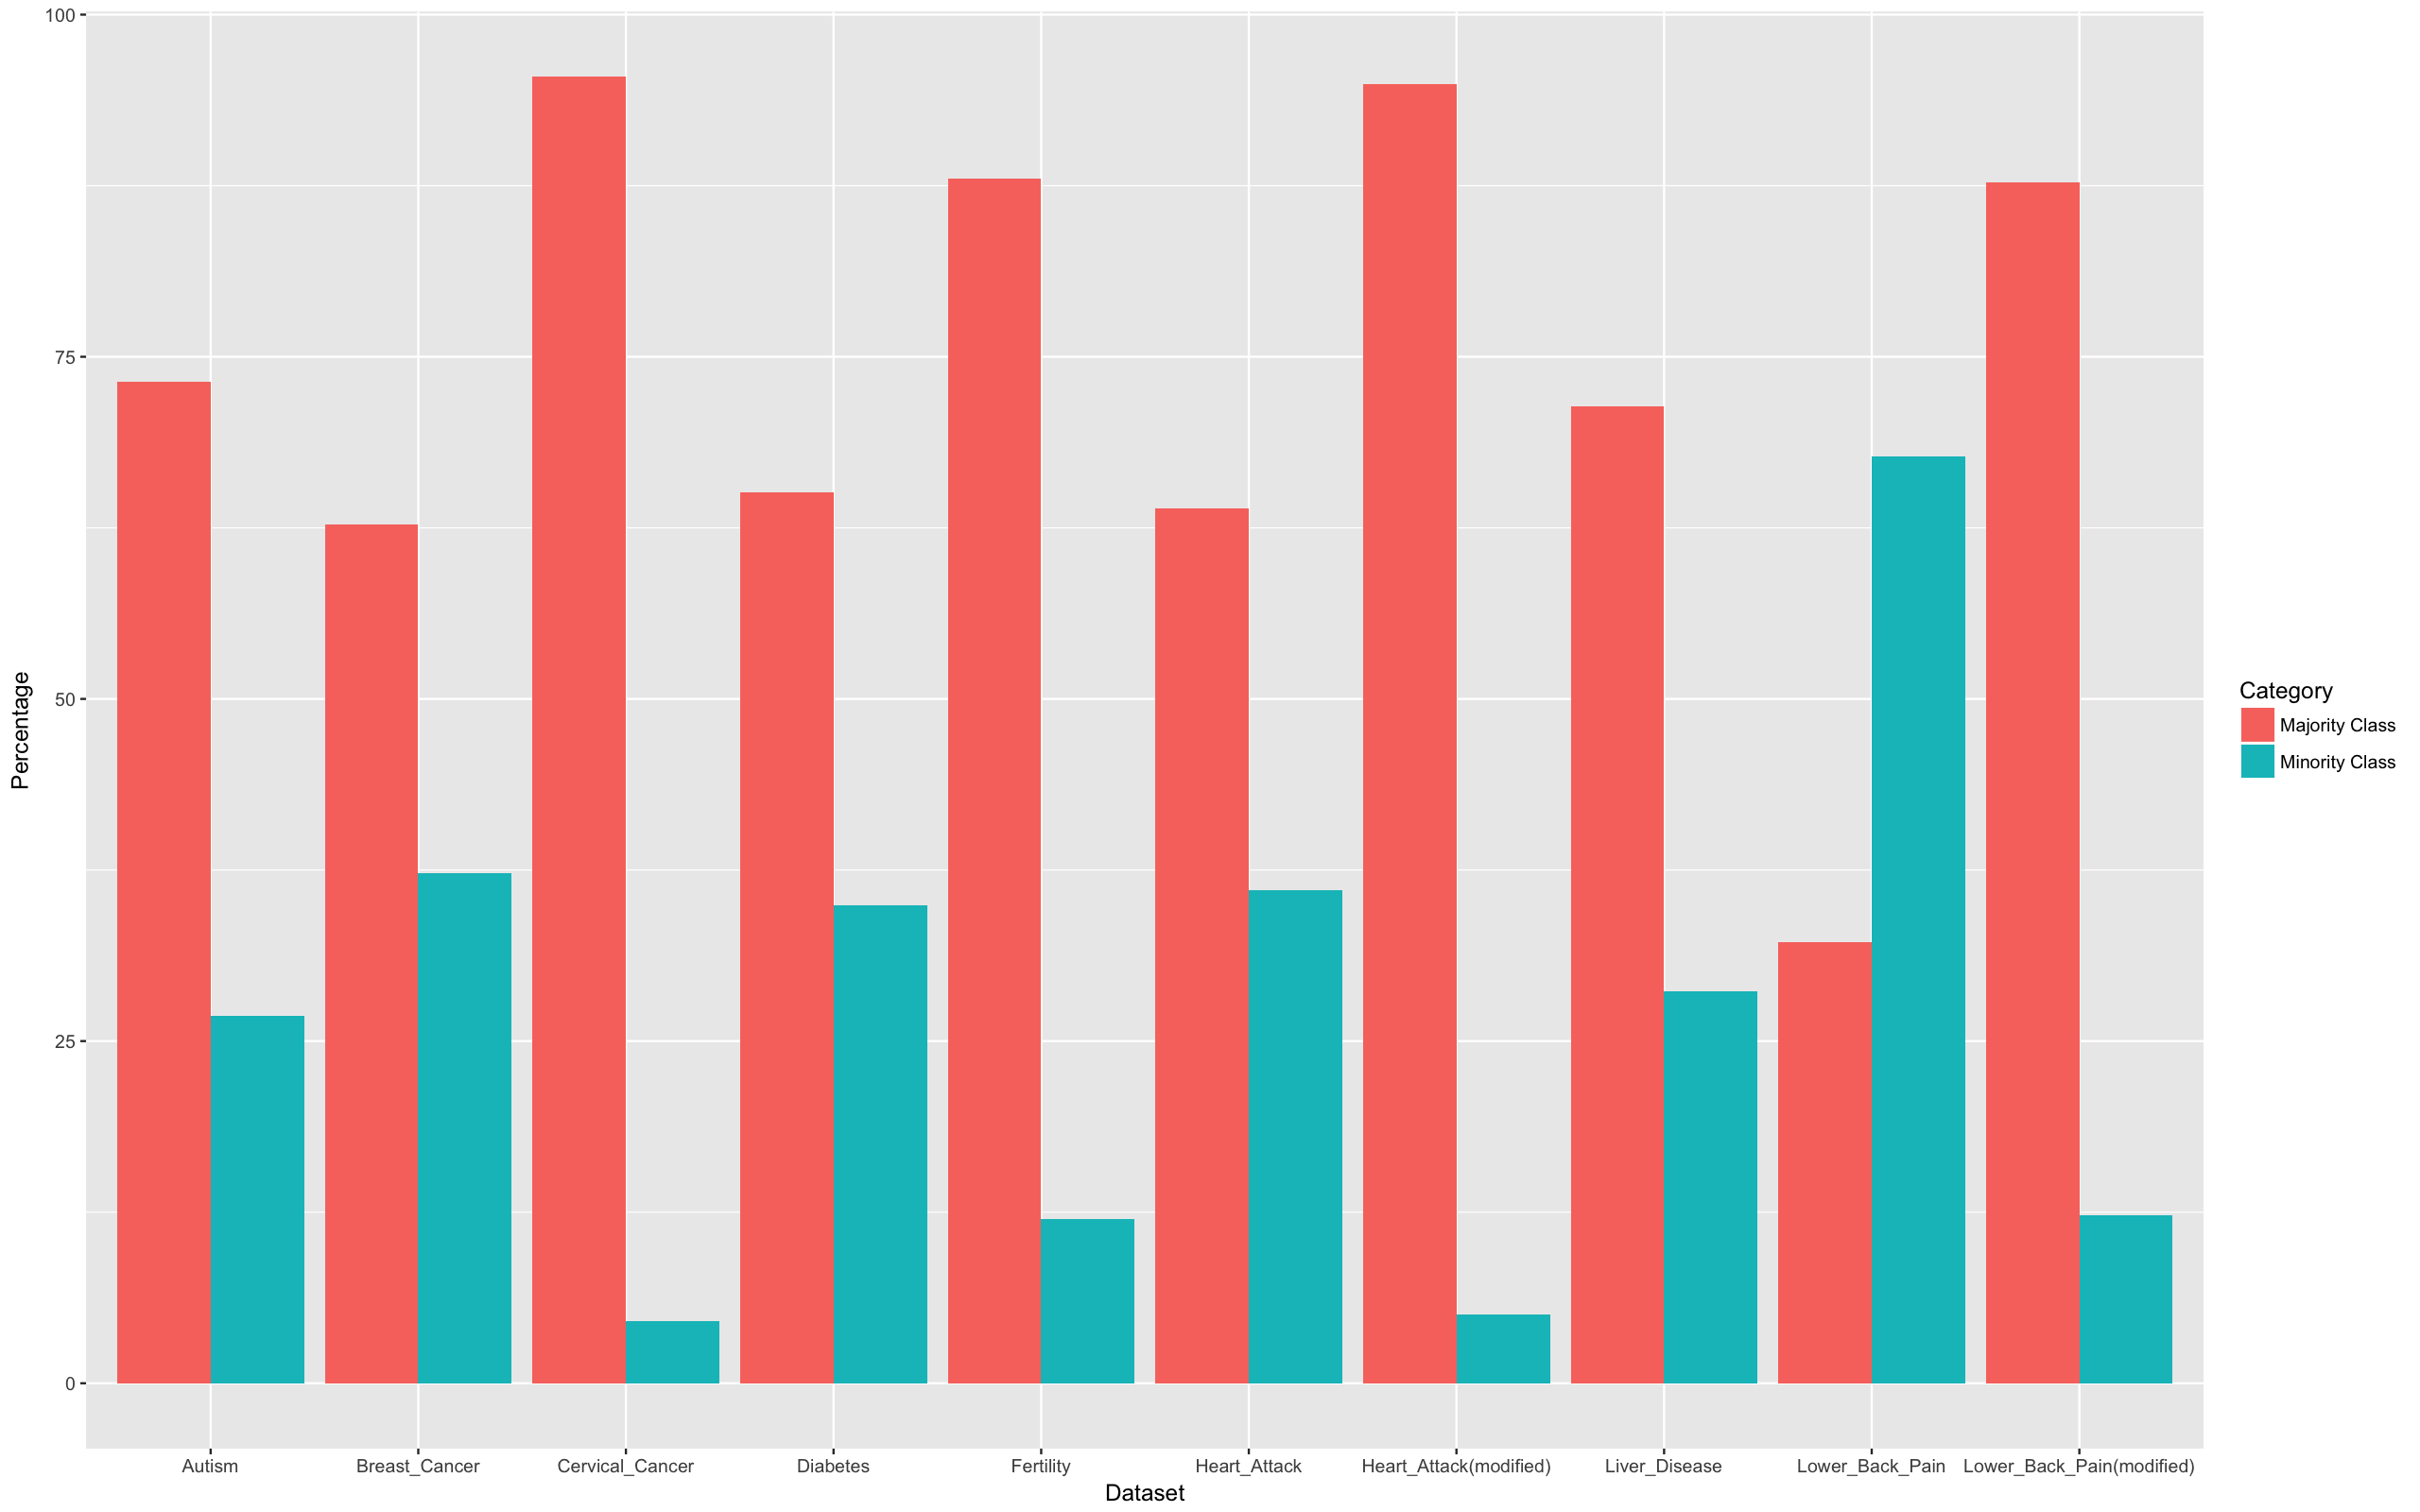
\includegraphics[width=0.8\textwidth]{ThesisTemplate/usingLatex/chapter4Images/figure4_1b.png}
    \caption{Class Distribution of the chosen datasets.\newline In all cases the majority class is the class representing healthy subjects and the minority class is the class representing affected subjects. In the case of the lower back pain dataset, the class representing the "abnormal" patients counts more instances than the the class representing the "normal" patients, however the terms minority and majority were kept for consistency with the other datasets.}
    \label{fig:my_label}
\end{figure}
\section{Modelling the datasets}
\subsection{Random Forest}
\begin{table}[ht]
\centering
\begin{tabular}{lrrrr}
  \hline
Dataset & Accuracy & Sensitivity & Precision & F1Score \\ 
  \hline
AuSDf & 100.00 & 1.00 & 1.00 & 1.00 \\ 
  BCDf & 91.67 & 0.86 & 0.94 & 0.89 \\ 
  CCDf & 93.75 & 0.33 & 0.45 & 0.38 \\ 
  DiabetesDf & 74.12 & 0.56 & 0.72 & 0.63 \\ 
  FertDf & 93.10 & 0.00 &  &  \\ 
  HAPDf & 90.80 & 0.83 & 0.89 & 0.86 \\ 
  LBPDf & 81.52 & 0.90 & 0.84 & 0.87 \\ 
  LiverDf & 71.68 & 0.35 & 0.58 & 0.44 \\ 
   \hline
\end{tabular}
\end{table}
\subsection{Support Machine Vector}
\subsection{K-Nearest Neighbour}
\subsection{Naive  Bayes}
\section{Modelling the datasets with data-level solutions applied}
\subsection{Undersampling of the majority class}
undersampling majority class 40\%
\begin{table}[ht]
\centering
\begin{tabular}{lrrrr}
  \hline
Dataset & Accuracy & Sensitivity & Precision & F1Score \\ 
  \hline
AuSDf & 100.00 & 1.00 & 1.00 & 1.00 \\ 
  BCDf & 94.23 & 0.98 & 0.93 & 0.96 \\ 
  CCDf & 95.45 & 0.75 & 0.82 & 0.78 \\ 
  DiabetesDf & 69.06 & 0.88 & 0.62 & 0.73 \\ 
  FertDf & 92.31 & 0.67 & 1.00 & 0.80 \\ 
  HAPDf & 81.13 & 0.90 & 0.80 & 0.85 \\ 
  LBPDf & 93.06 & 1.00 & 0.92 & 0.96 \\ 
  LiverDf & 70.71 & 0.86 & 0.62 & 0.72 \\ 
   \hline
\end{tabular}
\end{table}

undersampling majority class 60\%
\begin{table}[ht]
\centering
\begin{tabular}{lrrrr}
  \hline
Dataset & Accuracy & Sensitivity & Precision & F1Score \\ 
  \hline
AuSDf & 100.00 & 1.00 & 1.00 & 1.00 \\ 
  BCDf & 96.03 & 0.94 & 0.98 & 0.96 \\ 
  CCDf & 92.50 & 0.61 & 0.69 & 0.65 \\ 
  DiabetesDf & 70.24 & 0.78 & 0.65 & 0.71 \\ 
  FertDf & 77.78 & 0.00 & 0.00 &  \\ 
  HAPDf & 79.69 & 0.69 & 0.92 & 0.79 \\ 
  LBPDf & 78.75 & 0.92 & 0.82 & 0.86 \\ 
  LiverDf & 64.75 & 0.46 & 0.54 & 0.49 \\ 
   \hline
\end{tabular}
\end{table}

undersampling majority class 75\%
\begin{table}[ht]
\centering
\begin{tabular}{lrrrr}
  \hline
Dataset & Accuracy & Sensitivity & Precision & F1Score \\ 
  \hline
AuSDf & 100.00 & 1.00 & 1.00 & 1.00 \\ 
  BCDf & 95.10 & 0.90 & 1.00 & 0.95 \\ 
  CCDf & 95.38 & 0.74 & 0.78 & 0.76 \\ 
  DiabetesDf & 75.26 & 0.64 & 0.70 & 0.67 \\ 
  FertDf & 85.71 & 0.50 & 0.33 & 0.40 \\ 
  HAPDf & 83.33 & 0.75 & 0.81 & 0.78 \\ 
  LBPDf & 86.90 & 0.94 & 0.90 & 0.92 \\ 
  LiverDf & 61.70 & 0.31 & 0.52 & 0.39 \\ 
   \hline
\end{tabular}
\end{table}


\subsection{Oversampling of the minority class}
Oversampling using SMOTE (retain majority class, oversample 100\%)
100, 400
table showing training set distribution before and after smote
\begin{table}[ht]
\centering
\begin{tabular}{lrrrr}
  \hline
Dataset & MajorityClass & MinorityClass & NewMajorityClass & NewMinorityClass \\ 
  \hline
AuSDf & 353 & 140 & 560 & 280 \\ 
  BCDf & 258 & 143 & 572 & 286 \\ 
  CCDf & 573 &  29 & 116 &  58 \\ 
  DiabetesDf & 362 & 178 & 712 & 356 \\ 
  FertDf &  61 &  10 &  40 &  20 \\ 
  HAPDf & 131 &  76 & 304 & 152 \\ 
  LBPDf &  71 & 147 & 142 & 284 \\ 
  LiverDf & 297 & 113 & 452 & 226 \\ 
  subHAPDf & 134 &   7 &  28 &  14 \\ 
  subLBPDf &  74 &   8 &  32 &  16 \\ 
   \hline
\end{tabular}
\end{table}


\begin{table}[ht]
\centering
\begin{tabular}{lrrrr}
  \hline
Dataset & Accuracy & Sensitivity & Precision & F1Score \\ 
  \hline
AuSDf & 100.00 & 1.00 & 1.00 & 1.00 \\ 
  BCDf & 93.45 & 0.90 & 0.94 & 0.92 \\ 
  CCDf & 97.66 & 0.90 & 0.64 & 0.75 \\ 
  DiabetesDf & 75.00 & 0.62 & 0.71 & 0.66 \\ 
  FertDf & 75.86 & 0.50 & 0.14 & 0.22 \\ 
  HAPDf & 88.51 & 0.83 & 0.83 & 0.83 \\ 
  LBPDf & 78.26 & 0.84 & 0.84 & 0.84 \\ 
  LiverDf & 71.10 & 0.56 & 0.54 & 0.55 \\ 
  subHAPDf & 92.98 & 0.33 & 0.33 & 0.33 \\ 
  subLBPDf & 93.75 & 0.67 & 1.00 & 0.80 \\ 
   \hline
\end{tabular}
\end{table}


Repeat experiment to exclude modified heart attack and lowback pain dataset and do smote on those separately
\begin{table}[ht]
\centering
\begin{tabular}{lrrrr}
  \hline
Dataset & MajorityClass & MinorityClass & NewMajorityClass & NewMinorityClass \\ 
  \hline
AuSDf & 353 & 140 & 560 & 280 \\ 
  BCDf & 258 & 143 & 572 & 286 \\ 
  CCDf & 573 &  29 & 116 &  58 \\ 
  DiabetesDf & 362 & 178 & 712 & 356 \\ 
  FertDf &  61 &  10 &  40 &  20 \\ 
  HAPDf & 131 &  76 & 304 & 152 \\ 
  LBPDf &  71 & 147 & 142 & 284 \\ 
  LiverDf & 297 & 113 & 452 & 226 \\ 
   \hline
\end{tabular}
\end{table}

\begin{table}[ht]
\centering
\begin{tabular}{lrrrr}
  \hline
Dataset & Accuracy & Sensitivity & Precision & F1Score \\ 
  \hline
AuSDf & 100.00 & 1.00 & 1.00 & 1.00 \\ 
  BCDf & 93.45 & 0.90 & 0.94 & 0.92 \\ 
  CCDf & 97.66 & 0.90 & 0.64 & 0.75 \\ 
  DiabetesDf & 75.00 & 0.62 & 0.71 & 0.66 \\ 
  FertDf & 75.86 & 0.50 & 0.14 & 0.22 \\ 
  HAPDf & 88.51 & 0.83 & 0.83 & 0.83 \\ 
  LBPDf & 78.26 & 0.84 & 0.84 & 0.84 \\ 
  LiverDf & 71.10 & 0.56 & 0.54 & 0.55 \\ 
   \hline
\end{tabular}
\end{table}

Now do RF on HA and LBP
\begin{table}[ht]
\centering
\begin{tabular}{lrrrr}
  \hline
Dataset & MajorityClass & MinorityClass & NewMajorityClass & NewMinorityClass \\ 
  \hline
subHAPDf & 134 &   7 &  84 &  21 \\ 
  subLBPDf &  74 &   8 &  96 &  24 \\ 
   \hline
\end{tabular}
\end{table}

\begin{table}[ht]
\centering
\begin{tabular}{lrrrr}
  \hline
Dataset & Accuracy & Sensitivity & Precision & F1Score \\ 
  \hline
subHAPDf & 92.98 & 0.33 & 0.33 & 0.33 \\ 
  subLBPDf & 87.50 & 0.33 & 1.00 & 0.50 \\ 
   \hline
\end{tabular}
\end{table}

do fertility on its own
\begin{table}[ht]
\centering
\begin{tabular}{lrrrr}
  \hline
Dataset & MajorityClass & MinorityClass & NewMajorityClass & NewMinorityClass \\ 
  \hline
FertDf &  61 &  10 & 120 &  30 \\ 
   \hline
\end{tabular}
\end{table}

\begin{table}[ht]
\centering
\begin{tabular}{lrrrr}
  \hline
Dataset & Accuracy & Sensitivity & Precision & F1Score \\ 
  \hline
FertDf & 96.55 & 0.50 &   1 & 0.67 \\ 
   \hline
\end{tabular}
\end{table}


\subsection{k-mean}

\section{Conclusions}

The main conclusions for this chapter.


